%%%%%%%%%%%%%%%%%%%%%%%%%%%%%%%%%%%%%%%%%%%%%%%%%%%%%%%%%%%%%%%%%%%%%%%%%%%%%%%%%%%%%%%%%%%%%%%%%%%%%%%%%%%%%%%%%%%%%%%%
\newpage
\chapter {\Large{Database API's}}


\section{Data Types}
Based on java variable type siminov decides the data type of column.

\begin{enumerate}

	\item \small \textbf{int}: Java int primitive data type is converted to \textbf{INTEGER} Sqlite data type.

		\par
		\textbf{Example:} Java int  Primitive Data Type
			\lstinputlisting[language=Java]{Resources/data_type_int_primitive_example.txt}

	\item \small \textbf{Integer}: Java Integer class data type is converted to \textbf{INTEGER} Sqlite data type.

		\par
		\textbf{Example:} Java Integer Class Data Type
			\lstinputlisting[language=Java]{Resources/data_type_integer_class_example.txt}

	\item \small \textbf{long}: Java long primitive data type is converted to \textbf{INTEGER} Sqlite data type.

		\par
		\textbf{Example:} Java long Primitive Data Type
			\lstinputlisting[language=Java]{Resources/data_type_long_primitive_example.txt}

	\item \small \textbf{Long}: Java Long class data type is converted to \textbf{INTEGER} Sqlite data type.

		\par
		\textbf{Example:} Java Long Class Data Type
			\lstinputlisting[language=Java]{Resources/data_type_long_class_example.txt}

	\item \small \textbf{float}: Java float primitive data type is converted to \textbf{REAL} Sqlite data type.

		\par
		\textbf{Example:} Java float Primitive Data Type
			\lstinputlisting[language=Java]{Resources/data_type_float_primitive_example.txt}

	\item \small \textbf{Float}: Java Float class data type is converted to \textbf{REAL} Sqlite data type.

		\par
		\textbf{Example:} Java Float Class Data Type
			\lstinputlisting[language=Java]{Resources/data_type_float_class_example.txt}

	\item \small \textbf{boolean}: Java boolean primitive data type is converted to \textbf{NUMERIC} Sqlite data type.

		\par
		\textbf{Example:} Java boolean Primitive Data Type
			\lstinputlisting[language=Java]{Resources/data_type_boolean_primitive_example.txt}

	\item \small \textbf{Boolean}: Java Boolean class data type is converted to \textbf{NUMERIC} Sqlite data type.

		\par
		\textbf{Example:} Java Boolean Class Data Type
			\lstinputlisting[language=Java]{Resources/data_type_boolean_class_example.txt}

	\item \small \textbf{char}: Java char array primitive data type is converted to \textbf{TEXT} Sqlite data type.

		\par
		\textbf{Example:} Java char Array Primitive Data Type
			\lstinputlisting[language=Java]{Resources/data_type_char_example.txt}

	\item \small \textbf{Character}: Java Character class data type is converted to \textbf{TEXT} Sqlite data type.

		\par
		\textbf{Example:} Java Character Class Data Type
			\lstinputlisting[language=Java]{Resources/data_type_character_class_example.txt}

	\item \small \textbf{String}: Java String class data type is converted to \textbf{TEXT} Sqlite data type.

		\par
		\textbf{Example:} Java String Class Data Type
			\lstinputlisting[language=Java]{Resources/data_type_string_class_example.txt}

	\item \small \textbf{byte}: Java byte array data type is converted to \textbf{NONE} Sqlite data type.

		\par
		\textbf{Example:} Java byte Array Primitive Data Type
			\lstinputlisting[language=Java]{Resources/data_type_byte_primitive_example.txt}

	\item \small \textbf{Byte}: Java Byte class data type is converted to \textbf{NONE} Sqlite data type.

		\par
		\textbf{Example:} Java Byte Class Data Type
			\lstinputlisting[language=Java]{Resources/data_type_byte_class_example.txt}

	\item \small \textbf{void}: Java void primitive data type is converted to \textbf{NONE} Sqlite data type.

		\par
		\textbf{Example:} Java void Primitive Data Type
			\lstinputlisting[language=Java]{Resources/data_type_void_primitive_example.txt}

	\item \small \textbf{Void}: Java Void class data type is converted to \textbf{NONE} Sqlite data type.

		\par
		\textbf{Example:} Java Void Class Data Type
			\lstinputlisting[language=Java]{Resources/data_type_void_class_example.txt}

	\item \small \textbf{short}: Java short primitive is convered to \textbf{INTEGER} Sqlite data type.

		\par
		\textbf{Example:} Java short Primitive Data Type
			\lstinputlisting[language=Java]{Resources/data_type_short_primitive_example.txt}

	\item \small \textbf{Short}: Java Short class data type is converted to \textbf{INTEGER} Sqlite data type.
		
		\par
		\textbf{Example:} Java Short Class Data Type
			\lstinputlisting[language=Java]{Resources/data_type_short_class_example.txt}

\end{enumerate}


\par
Sqlite data types:
	
\begin{enumerate}

	\item \small \textbf{INTEGER Sqlite Data Type}: This sqlite data type generaly contain \textit{INT}, \textit{INTEGER}, \textit{TINYINT}, \textit{SMALLINT}, \textit{MEDIUMINT}, \textit{BIGINT}, \textit{UNSIGNED BIG INT}, \textit{INT2}, \textit{INT8}.
	
	\item \small \textbf{TEXT Sqlite Data Type}: This sqlite data type generaly contain \textit{CHARACTER(20)}, \textit{VARCHAR(255)}, \textit{VARYING CHARACTER(255)}, \textit{NCHAR(55)}, \textit{NATIVE CHARACTER(70)}, \textit{NVARCHAR(100)}, \textit{TEXT}, \textit{CLOB}.

	\item \small \textbf{REAL Sqlite Data Type}: This sqlite data type generaly contain \textit{REAL}, \textit{DOUBLE}, \textit{DOUBLE PRECISION}, \textit{FLOAT}.
	
	\item \small \textbf{NONE Sqlite Data Type}: This sqlite data type generaly contain \textit{BLOB}, \textit{NO DATA TYPE SPECIFIED}.

	\item \small \textbf{NUMERIC Sqlite Data Type}: This sqlite data type generaly contain \textit{NUMERIC}, \textit{DECIMAL(10,5)}, \textit{BOOLEAN}, \textit{DATE}, \textit{DATETIME}.

\end{enumerate}


					\begin{center}
						\colorbox{grey}{
						\parbox[t]{.8\linewidth}{
							\fontsize{11pt}{11pt}\selectfont % The first argument for fontsize is the font size of the text and the second is the line spacing - you may need to play with these for your particular title
							\vspace*{0.1cm} % Space between the start of the title and the top of the grey box
		
							\hfill \textbf{Note} \\
							If you define ORM using Annotation then you dont have to specify data type, it will automatically be configured based on variable data type.
				
							\vspace*{0.0cm} % Space between the end of the title and the bottom of the grey box
						}
					}

					\end{center}



\section{Database API's}
	
	\subsection{Create Database}Siminov provides APIs to create database, based on schema defined in DatabaseDescriptor.si.xml file.

			\textbf{API:} Basically Use IDatabase Interface
				\lstinputlisting[language=Java]{Resources/create_database_api.txt}
		
					\begin{center}
						\colorbox{grey}{
						\parbox[t]{.8\linewidth}{
							\fontsize{11pt}{11pt}\selectfont % The first argument for fontsize is the font size of the text and the second is the line spacing - you may need to play with these for your particular title
							\vspace*{0.1cm} % Space between the start of the title and the top of the grey box
		
							\hfill \textbf{Note} \\
							Generally database creation will be automatically handled by Siminov, but you can do it manually also.

							\textbf{Example:} Manually Creating Database.
								\lstinputlisting[language=Java]{Resources/create_database_api_example.txt}

							\vspace*{0.0cm} % Space between the end of the title and the bottom of the grey box
						}
					}

					\end{center}


	\subsection{Drop Database}Database class provides API to drop complete database of an application.

		\textbf{API}: Drop Database.
		\lstinputlisting[language=Java]{Resources/drop_database_api.txt}
		

		\textbf{Example}
		\lstinputlisting[language=Java]{Resources/drop_database_api_example.txt}



	\subsection{Create Table}Using this API you can create table on database.

			\begin{center}
				\colorbox{grey}{
				\parbox[t]{.8\linewidth}{
					\fontsize{11pt}{11pt}\selectfont % The first argument for fontsize is the font size of the text and the second is the line spacing - you may need to play with these for your particular title
					\vspace*{0.1cm} % Space between the start of the title and the top of the grey box

					\hfill \textbf{Note} \\
					Generally database and its table creation will automatically be handled by Siminov, but u can do it manually also.

					\vspace*{0.0cm} % Space between the end of the title and the bottom of the grey box
					}
			}

			\end{center}


		\par
		There are three ways to create table in database.

		\begin{enumerate}

			\item \small \textbf{Defining table structure using DatabaseMappingDescriptor.si.xml file}

				\textbf{Example}: Liquor.si.xml file Of Siminov Template Application.
				\lstinputlisting[language=XML]{Resources/create_table_example_xml.txt}
		
			\item \small \textbf{Defining table structure using Annotations}

				\textbf{Example}: Liquor Class Of Siminov Template Application.
				\lstinputlisting[language=Java]{Resources/create_table_example_xml_annotation.txt}

			\item \small \textbf{Creating table programmatically}

				\textbf{Example}: Creating Liquor Table Programmatically.
				\lstinputlisting[language=Java]{Resources/create_table_example_programmatically.txt}

		\end{enumerate}


		\par
		 Siminov \textbf{Database} class provide few APIs to create table programmtically.

		\begin{enumerate}

			\item \small \lstinputlisting[language=Java]{Resources/create_table_iterator_of_database_mapping_descriptor_objects.txt}

				\par
				Example:
				\lstinputlisting[language=Java]{Resources/create_table_iterator_of_database_mapping_descriptor_objects_example.txt}

	
			\item \small \lstinputlisting[language=Java]{Resources/create_table_database_mapping_object.txt}

				\par
				Example: Creating Liquor Table Programmatically.
				\lstinputlisting[language=Java]{Resources/create_table_database_mapping_object_example.txt}

		
		\end{enumerate}


	\subsection{Drop Table} Database class provides following API's to drop a table.

		\begin{enumerate}

			\item \small \lstinputlisting[language=Java]{Resources/instance_drop_table_method.txt}

				\par
				\textbf{Example}: Drop Liquor Table Through Liquor Class Object.
				\lstinputlisting[language=Java]{Resources/instance_drop_table_method_example.txt}

			\item \small \lstinputlisting[language=Java]{Resources/static_drop_table_method.txt}

				\par
				\textbf{Example}: Drop Liquor Table Using Static API Of Database.
				\lstinputlisting[language=Java]{Resources/static_drop_table_method_example.txt}

		\end{enumerate}
		

	\subsection{Create Index}
		
		\par
		There are two ways to create index.

		\begin{enumerate}
		
			\item \small \textbf{Define Index Structure Using DatabaseMappingDescriptor.si.xml file}
				\lstinputlisting[language=Java]{Resources/create_index_using_xml.txt}
								
	
			\item \small \textbf{Creating Index Programmatically}
				\par 
				Database class provides few API's two create index programmatically

				\begin{enumerate}

					\item \small \lstinputlisting[language=Java]{Resources/create_index_programmatically_1.txt}

						\par
						\textbf{Example}: 
							\lstinputlisting[language=Java]{Resources/create_index_programmatically_1_example.txt}

					\item \small \lstinputlisting[language=Java]{Resources/create_index_programmatically_2.txt}

						\par
						\textbf{Example}: 
							\lstinputlisting[language=Java]{Resources/create_index_programmatically_2_example.txt}

					\item \small \lstinputlisting[language=Java]{Resources/create_index_programmatically_3.txt}

						\par
						\textbf{Example}:
							\lstinputlisting[language=Java]{Resources/create_index_programmatically_3_example.txt}

					\item \small \lstinputlisting[language=Java]{Resources/create_index_programmatically_4.txt}

						\par
						\textbf{Example}:
							\lstinputlisting[language=Java]{Resources/create_index_programmatically_4_example.txt}

				\end{enumerate}
			

		\end{enumerate}

	\subsection{Drop Index}
		\par 
		Database class provides following API's to drop index from table.
		
		\begin{enumerate}

			\item \small \lstinputlisting[language=Java]{Resources/drop_index_1.txt}

				\par
				\textbf{Example}:
					\lstinputlisting[language=Java]{Resources/drop_index_1_example.txt}

			\item \small \lstinputlisting[language=Java]{Resources/drop_index_2.txt}

				\par
				\textbf{Example}:
					\lstinputlisting[language=Java]{Resources/drop_index_2_example.txt}

		\end{enumerate}
		

	\subsection{Select}

		\par
		Database class provides following API's to fetch tuples from table.

		\begin{enumerate}

			\item \small \lstinputlisting[language=Java]{Resources/select.txt}

				\par
				Fetch tuples from table.

				\textbf{IFetch}: Exposes API's to provide information based on which tuples will be fetched from table.
					\lstinputlisting[language=Java]{Resources/ifetch_interface.txt}
	
			
				\textbf{IFetchClause}: Exposes API's to provide condition to where clause based on which tuples will be fetched from table.
					\lstinputlisting[language=Java]{Resources/ifetchclause_interface.txt}

				\textbf{Example}: Select Liquor Where Type Equal To RUM
					\lstinputlisting[language=Java]{Resources/select_example.txt}

			\item \small \lstinputlisting[language=Java]{Resources/manual_select.txt}

				\par
				Returns all tuples based on manual query from mapped table for invoked class object.

				\textbf{Example}: Select Liquor Object.
					\lstinputlisting[language=Java]{Resources/manual_select_example.txt}


		\end{enumerate}



	\subsection{Save}
		\lstinputlisting[language=Java]{Resources/save.txt}

			\par
			\textbf{Example}: Saving Liquor Object.
				\lstinputlisting[language=Java]{Resources/save_example.txt}


	\subsection{Update}
		\lstinputlisting[language=Java]{Resources/update.txt}

			\par
			\textbf{Example}: Updaing Liquor Object.
				\lstinputlisting[language=Java]{Resources/update_example.txt}


	\subsection{Save Or Update}
		\lstinputlisting[language=Java]{Resources/save_or_update.txt}

			\par
			\textbf{Example}: Save Or Update Liquor Object.
				\lstinputlisting[language=Java]{Resources/save_or_update_example.txt}



			\begin{center}
				\colorbox{grey}{
				\parbox[t]{.8\linewidth}{
					\fontsize{11pt}{11pt}\selectfont % The first argument for fontsize is the font size of the text and the second is the line spacing - you may need to play with these for your particular title
					\vspace*{0.1cm} % Space between the start of the title and the top of the grey box

					\hfill \textbf{Note} \\
					If tuple is not present in table then it will insert it into table else it will update the tuple.

					\vspace*{0.0cm} % Space between the end of the title and the bottom of the grey box
					}
			}

			\end{center}


	\subsection{Delete}
		\par 
		Database class provides following API's to delete tuples from table.

			\textbf{API}: Delete API.
				\lstinputlisting[language=Java]{Resources/delete.txt}
		
			\textbf{IDelete}:  Exposes API's to delete tuples from table.

				\lstinputlisting[language=Java]{Resources/idelete.txt}

			
			\textbf{IDeleteClause}: Exposes API's to provide condition on where clause to delete tuple from table.
				\lstinputlisting[language=Java]{Resources/ideleteclause.txt}

			\textbf{Example}: 
				\lstinputlisting[language=Java]{Resources/delete_example.txt}
	

\section{Database Siminov API's}


	\subsection{Get Database Descriptor}
	\lstinputlisting[language=Java]{Resources/get_database_descriptor.txt}

				\par
				\textbf{Example}: Get Database Descriptor Object Which Contain Liquor Table.
					\lstinputlisting[language=Java]{Resources/get_database_descriptor_example.txt}


	\subsection{Get Database Mapping Descriptor}
	\lstinputlisting[language=Java]{Resources/get_database_mapping.txt}

				\par
				\textbf{Example}: Get Database Mapping Descriptor Object Related To Liquor Table.
					\lstinputlisting[language=Java]{Resources/get_database_mapping_example.txt}


	\subsection{Get Table Name}
	\lstinputlisting[language=Java]{Resources/get_table_name.txt}

				\par
				\textbf{Example}: Get Liquor Object Table Name.
					\lstinputlisting[language=Java]{Resources/get_table_name_example.txt}
		

	\subsection{Get Column Names}
	\lstinputlisting[language=Java]{Resources/get_column_names.txt}

				\par
				\textbf{Example}: Get All Column Names Of Liquor Table.
					\lstinputlisting[language=Java]{Resources/get_column_names_example.txt}


	\subsection{Get Column Values}
	\lstinputlisting[language=Java]{Resources/get_column_values.txt}

				\par
				\textbf{Example}: Get All Column Values Of Liquor Object.
					\lstinputlisting[language=Java]{Resources/get_column_values_example.txt}


	\subsection{Get Column Types}
	\lstinputlisting[language=Java]{Resources/get_column_types.txt}

				\par
				\textbf{Example}: Get All Column Types Of Liquor Table.
					\lstinputlisting[language=Java]{Resources/get_column_types_example.txt}


	\subsection{Get Primary Keys}
	\lstinputlisting[language=Java]{Resources/get_primary_keys.txt}

				\par
				\textbf{Example}: Get All Primary Keys Of Liquor Table.
					\lstinputlisting[language=Java]{Resources/get_primary_keys_example.txt}


	\subsection{Get Mandatory Fields}
	\lstinputlisting[language=Java]{Resources/get_mandatory_fields.txt}

				\par
				\textbf{Example}: Get All Column Names Which Are Marked As Manadatory Fields.
					\lstinputlisting[language=Java]{Resources/get_mandatory_fields_example.txt}

	\subsection{Get Unique Fields}
	\lstinputlisting[language=Java]{Resources/get_unique_fields.txt}

				\par
				\textbf{Example}: Get All Column Names Which Are Marked As Unique.
					\lstinputlisting[language=Java]{Resources/get_unique_fields_example.txt}


	\subsection{Get Foreign Keys}
	\lstinputlisting[language=Java]{Resources/get_foreign_keys.txt}

				\par
				\textbf{Example}: Get All Column Names Which Are Marked As Foreign Keys.
					\lstinputlisting[language=Java]{Resources/get_foreign_keys_example.txt}


\section{Database Aggregation API's}


	\subsection{Count}
		\par
		Returns the count of rows based on information provided.

			\textbf{API}: Count API.
				\lstinputlisting[language=Java]{Resources/count.txt}
		
			\textbf{ICount}:  Exposes API's to get count of the number of times that X is not NULL in a group.
						 The count(*) function (with no arguments) returns the total number of rows in the group.

				\lstinputlisting[language=Java]{Resources/icount_interface.txt}

			
			\textbf{ICountClause}: Exposes API's to provide condition on where clause to calculate count.
				\lstinputlisting[language=Java]{Resources/icountclause_interface.txt}

			\textbf{Example}: Get count of liquors type equal to RUM.
				\lstinputlisting[language=Java]{Resources/count_example.txt}


	\subsection{Average} 
		\par 
		Returns the average based on column name provided.

			\textbf{API}: Average API.
				\lstinputlisting[language=Java]{Resources/average.txt}
		
			\textbf{IAverage}:  Exposes API's to get average value of all non-NULL X within a group. 
 						 String and BLOB values that do not look like numbers are interpreted as 0.
						 The result of avg() is always a floating point value as long as at there is at least one non-NULL input even if all inputs are integers.
						 The result of avg() is NULL if and only if there are no non-NULL inputs.

				\lstinputlisting[language=Java]{Resources/iaverage_interface.txt}

			
			\textbf{IAverageClause}: Exposes API's to provide condition on where clause to calculate average.
				\lstinputlisting[language=Java]{Resources/iaverageclause_interface.txt}

			\textbf{Example}: 
				\lstinputlisting[language=Java]{Resources/average_example.txt}
		

	\subsection{Sum} 
		\par 
		Returns the sum based on column name provided.

			\textbf{API}: Sum API.
				\lstinputlisting[language=Java]{Resources/sum.txt}
		
			\textbf{ISum}:   Exposes API's to return sum of all non-NULL values in the group.
					  	 If there are no non-NULL input rows then sum() returns NULL but total() returns 0.0.
						 NULL is not normally a helpful result for the sum of no rows but the SQL standard requires it and most other SQL database engines implement sum() that way so SQLite does it in the same way in order to be compatible.
						 The result of sum() is an integer value if all non-NULL inputs are integers. 

				\lstinputlisting[language=Java]{Resources/isum_interface.txt}

			
			\textbf{ISumClause}: Exposes API's to provide condition on where clause to calculate sum.
				\lstinputlisting[language=Java]{Resources/isumclause_interface.txt}

			\textbf{Example}: 
				\lstinputlisting[language=Java]{Resources/sum_example.txt}


	\subsection{Total} 
		\par 
		Returns the total based on column name provided.

			\textbf{API}: Total API.
				\lstinputlisting[language=Java]{Resources/total.txt}
		
			\textbf{ITotal}:     Exposes API's to return total of all non-NULL values in the group.
 						The non-standard total() function is provided as a convenient way to work around this design problem in the SQL language.
						The result of total() is always a floating point value.


				\lstinputlisting[language=Java]{Resources/itotal_interface.txt}

			
			\textbf{ITotalClause}: Exposes API's to provide condition on where clause to calculate total.
				\lstinputlisting[language=Java]{Resources/itotalclause_interface.txt}

			\textbf{Example}: 
				\lstinputlisting[language=Java]{Resources/total_example.txt}


	\subsection{Minimum} 
		\par 
		Returns the minimum based on column name provided.

			\textbf{API}: Minimum API.
				\lstinputlisting[language=Java]{Resources/minimum.txt}
		
			\textbf{IMin}:      Exposes API's to returns the minimum non-NULL value of all values in the group.
						The minimum value is the first non-NULL value that would appear in an ORDER BY of the column.
						Aggregate min() returns NULL if and only if there are no non-NULL values in the group.


				\lstinputlisting[language=Java]{Resources/iminimum_interface.txt}

			
			\textbf{IMinClause}: Exposes API's to provide condition on where clause to calculate minimum.
				\lstinputlisting[language=Java]{Resources/iminimumclause_interface.txt}

			\textbf{Example}: 
				\lstinputlisting[language=Java]{Resources/minimum_example.txt}



	\subsection{Maximum} 
		\par 
		Returns the minimum based on column name provided.

			\textbf{API}: Maximum API.
				\lstinputlisting[language=Java]{Resources/maximum.txt}
		
			\textbf{IMax}:    Exposes API's to returns the maximum value of all values in the group.
						The maximum value is the value that would be returned last in an ORDER BY on the same column. 
						Aggregate max() returns NULL if and only if there are no non-NULL values in the group.


				\lstinputlisting[language=Java]{Resources/imax_interface.txt}

			
			\textbf{IMaxClause}: Exposes API's to provide condition on where clause to calculate maximum.
				\lstinputlisting[language=Java]{Resources/imaxclause_interface.txt}

			\textbf{Example}: 
				\lstinputlisting[language=Java]{Resources/maximum_example.txt}


	\subsection{Group Concat} 
		\par 
		Returns the group concat based on column name provided.

			\textbf{API}: Group Concat API.
				\lstinputlisting[language=Java]{Resources/groupconcat.txt}
		
			\textbf{IGroupConcat}:     Exposes API's to get group concat that returns a string which is the concatenation of all non-NULL values of X.
							If parameter Y is present then it is used as the separator between instances of X. A comma (",") is used as the separator if Y is omitted.
							The order of the concatenated elements is arbitrary.


				\lstinputlisting[language=Java]{Resources/igroupconcat_interface.txt}

			
			\textbf{IGroupConcatClause}: Exposes API's to provide condition on where clause to calculate group concat.
				\lstinputlisting[language=Java]{Resources/igroupconcatclause_interface.txt}

			\textbf{Example}: 
				\lstinputlisting[language=Java]{Resources/groupconcat_example.txt}


\section{Database Transaction API's}

	\subsection{Begin Transaction}
	\lstinputlisting[language=Java]{Resources/begin_transaction.txt}

	\par
	Begins a transaction in \textbf{EXCLUSIVE} mode.

	\par
	Transactions can be nested. When the outer transaction is ended all of the work done in that transaction and all of the nested transactions will be committed or rolled back. The changes will be rolled back if any transaction is ended without being marked as clean(by calling commitTransaction). Otherwise they will be committed.

				\par
				\textbf{Example}: Saving Liquor Within Transaction.
					\lstinputlisting[language=Java]{Resources/begin_transaction_example.txt}


	\subsection{Commit Transaction}
	\lstinputlisting[language=Java]{Resources/commit_transaction.txt}

	\par
	Marks the current transaction as successful. Finally it will End a transaction.

				\par
				\textbf{Example}: Save And Commt Liquor Transaction.
					\lstinputlisting[language=Java]{Resources/commit_transaction_example.txt}

	
	\subsection{End Transaction}
	\lstinputlisting[language=Java]{Resources/end_transaction.txt}

	\par
	End the current transaction.

				\par
				\textbf{Example}: End Transaction After Save And Commit Transaction.
					\lstinputlisting[language=Java]{Resources/end_transaction_example.txt}


\section{Making Transaction Thread Safe}
By default any transaction executed on database is not thread safe, android provides API to make all transaction thread-safe by using locks around critical sections. This is pretty expensive, so if you know that your DB will nly be used by a single thread then you should not use this in your application.

	\par
	\textbf{Android API}: setLockingEnabled Enable/Disable
		\lstinputlisting[language=Java]{Resources/andorid_transaction_set_locking_enabled_api.txt}

Configuring transaction thread-safe in Siminov. To enable/disable transaction thread-safe in Siminov you have to use property is\_locking\_required defined in DatabaseDescriptor.si.xml file.

		\par
		\textbf{Example:} Siminov Template Application DatabaseDescriptor.si.xml file.
		\begin{figure}[htbp]
			\centering
				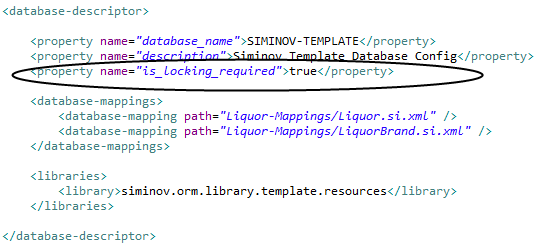
\includegraphics[height=7cm]{Resources/siminov_template_application_is_locking_enable_example.png}
		\end{figure}


\section{Preparing Where Clause}
Siminov does not provide any mechanism to prepare where-clause, Providing where-clause for fetch API is easy. It take same syntax as we form where-clause for SQLite statement.

\textbf{Example}: Fetch Liquor tuple where liquor type is Beer.
	\lstinputlisting[language=Java]{Resources/preparing_where_clause.txt}
	


\section{Handling Database Relationships}

	\subsection{One to One}
	One-To-One relationship is in which each row in one database table is linked to 1 and 1 other row in another table.

	\textbf{Example}: Relationship between Table A and Table B, each row in Table A is linked to another row in Table B. The number of rows in Table A must equal the number of rows in Table B.

	\textbf{One To One Syntax}: 
		\lstinputlisting[language=Java]{Resources/one_to_one_syntax.txt}

	\subsection{One to Many}
	One-To-Many relationship is in which each row in the related to table can be related to many rows in the relating table. This effectively save storage as the related record does not need to be stored multiple times in the relating table.

	\textbf{Example}: All the customers belonging to a business is stored in a customer table while all the customer invoices are stored in an invoice table. Each customer can have many invoices but each invoice can only be generated for a single customer.	
			
	\textbf{One To Many Syntax}: 
		\lstinputlisting[language=Java]{Resources/one_to_many_syntax.txt}

	\subsection{Many to One}
	Many-To-One relationship is in which one entity (typically a column or set of columns) contains values that refer to another entity (a column or set of columns) that has unique values.

	\textbf{Example}: In a geography schema having tables Region, State, and City, there are many states that are in a given region, but no states are in two regions.
	
	\textbf{Many To One Syntax}: 
		\lstinputlisting[language=Java]{Resources/many_to_one_syntax.txt}

	\subsection{Many to Many}
	Many-To-Many relationship is in which one or more rows in the table can be related to 0, 1 or many rows in another table. A mapping table is required in order to implement  such a relationship.

	\textbf{Example}: All the customers belonging to a bank is stored in a customer table while all the bank's products are stored in a product table. Each customer can have many products and each product can be assigned to many customers.
	
	\textbf{Many To Many Syntax}: 
		\lstinputlisting[language=Java]{Resources/many_to_many_syntax.txt}


